\documentclass[11pt]{article}

% ---------------------------------------------------------------------------
% The Value of the Marginal Solver
% Reflowed to the CVA CFP 2026 / Ledger journal house style (see README.md):
% Times New Roman 11.5/13.5, 3.1 cm side margins, 13 pt bold numbered section
% headings, inline italic em-dash subheadings, numbered superscript endnote
% citations in a "Notes and References" section.
% Single-author paper; first-person singular voice (academic-writing-style.md).
% ---------------------------------------------------------------------------

\usepackage[utf8]{inputenc}
\usepackage[T1]{fontenc}
\usepackage[a4paper,left=3.1cm,right=3.1cm,top=2.4cm,bottom=1.0cm,
            headheight=14pt,headsep=0.7cm,footskip=0.6cm]{geometry}
\usepackage{amsmath,amsthm}
\usepackage{newtxtext,newtxmath}   % Times New Roman-like text and math
\usepackage{booktabs}
\usepackage{graphicx}
\usepackage{microtype}
\usepackage[super,numbers,sort&compress]{natbib}
\usepackage[explicit]{titlesec}
\usepackage{fancyhdr}
\usepackage[hidelinks]{hyperref}

% --- Ledger body font size: 11.5 pt on 13.5 pt leading --------------------
\makeatletter
\renewcommand\normalsize{%
  \@setfontsize\normalsize{11.5pt}{13.5pt}%
  \abovedisplayskip 10\p@ \@plus3\p@ \@minus6\p@
  \belowdisplayskip \abovedisplayskip
  \abovedisplayshortskip \z@ \@plus3\p@
  \belowdisplayshortskip 6.5\p@ \@plus3.5\p@ \@minus3\p@}
\makeatother
\normalsize

% --- Section headings: 13 pt Times bold, numbered with a period -----------
\titleformat{\section}
  {\normalfont\bfseries\fontsize{13}{15}\selectfont}{\thesection.}{0.6em}{#1}
\titlespacing*{\section}{0pt}{2.2ex plus 1ex minus .2ex}{1.0ex}

% --- Numbered subheadings: inline, italic, followed by an em dash ----------
\titleformat{\subsection}[runin]
  {\normalfont\itshape}{\upshape\thesubsection}{0.5em}{#1}[\textup{---}]
\titlespacing*{\subsection}{0pt}{1.3ex plus .3ex}{0.15em}

% --- Run-in topic heads: inline, italic, followed by an em dash ------------
\titleformat{\paragraph}[runin]
  {\normalfont\itshape}{}{0pt}{#1}[\textup{---}]
\titlespacing*{\paragraph}{0pt}{1.1ex plus .2ex}{0.15em}

% --- Running head and page number (Ledger) --------------------------------
\pagestyle{fancy}
\fancyhf{}
\fancyhead[C]{\fontsize{10}{12}\selectfont CVA Academic Research Journal 2026}
\fancyfoot[L]{\fontsize{10}{12}\selectfont\thepage}
\renewcommand{\headrulewidth}{0pt}
\fancypagestyle{plain}{\fancyhf{}%
  \fancyhead[C]{\fontsize{10}{12}\selectfont CVA Academic Research Journal 2026}%
  \fancyfoot[L]{\fontsize{10}{12}\selectfont\thepage}%
  \renewcommand{\headrulewidth}{0pt}}

% References appear as a numbered "Notes and References" section (Ledger).
\renewcommand{\refname}{Notes and References}

\theoremstyle{plain}
\newtheorem{proposition}{Proposition}
\newtheorem{corollary}{Corollary}
\theoremstyle{definition}
\newtheorem{definition}{Definition}
\newtheorem{assumption}{Assumption}
\theoremstyle{remark}
\newtheorem{remark}{Remark}

\newcommand{\E}{\mathbb{E}}
\newcommand{\Prb}{\mathbb{P}}
\newcommand\blfootnote[1]{\begingroup\renewcommand\thefootnote{}%
  \footnotetext{#1}\addtocounter{footnote}{-1}\endgroup}

\begin{document}

% --- Title block (Ledger: 24 pt centered title, 13 pt author) --------------
\thispagestyle{plain}
\begin{center}
{\fontsize{24}{28}\selectfont The Value of the Marginal Solver:\\[2pt]
Competition and Best Execution\\ in Intent-Based Markets\par}
\vspace{1.4em}
{\fontsize{13}{16}\selectfont Nils Bundi\textsuperscript{*,\,1}\par}
\end{center}
\blfootnote{\fontsize{8}{9}\selectfont\textsuperscript{1}N.\ Bundi (\texttt{bund@zhaw.ch}) is a researcher at the Zurich University of Applied Sciences (ZHAW), Switzerland. \textsuperscript{*}Corresponding author.}
\vspace{0.4em}

% --- Abstract (Ledger: 10 pt, 1.2 cm side indents, bold run-in "Abstract.")
{\fontsize{10}{13}\selectfont
\setlength{\leftskip}{1.2cm}\setlength{\rightskip}{1.2cm}
\noindent\textbf{Abstract.}\quad Intent-based exchanges, the fastest-growing execution model in on-chain finance, replace order routing with a public solver auction. CoW Protocol is, to my knowledge, the first major exchange to publish the full competition behind each trade, winning and losing bids alike. I use that record to measure the counterfactual value of admitting more competitive bids to a customer order, order by order. Across its 565{,}259 auctions (twelve months, 692{,}964 orders, 47 solvers), a single retained bid leaves the median order about 14 basis points below its full field, a second closes most of the gap, and by roughly the fifth the marginal gain is under a basis point (auction-clustered bootstrap intervals throughout); the value of competition rises as liquidity thins. A protocol reward reform in the sample offers an institutional test rather than a clean experiment: three major solvers exited, rivals filled their place within a month, and margins conditional on participation changed little, patterns consistent with competition being supplied by the depth of the field rather than the identity of its members. Where a broker is bound to best execution by regulation, an intent exchange makes it observable as competition depth that anyone can recompute.
\par}

\vspace{0.7em}
{\fontsize{10}{13}\selectfont
\begin{center}KEY WORDS\end{center}
\vspace{-0.4em}
\begin{center}
1.~Solver competition.\quad 2.~Order flow auctions.\quad 3.~Best execution.\quad 4.~Batch auctions.\quad 5.~Market microstructure.
\end{center}
}
\vspace{0.5em}

\section{Introduction}

On-chain finance is rebuilding how trades are executed, and intent-based settlement has become its fastest-growing model. Rather than constructing and broadcasting a transaction, a user signs a declarative \emph{intent}, a desired outcome, and a network of professional \emph{solvers} competes in an auction to settle it on-chain. The design moves execution off the public mempool to shield users from the extractable value that arbitrage bots impose on transparent trading~\citep{daian2020flashboys}, a frequent batch auction~\citep{budish2015hft} rebuilt as a smart contract; it now spans CoW Protocol, UniswapX, and 1inch Fusion, and CoW alone settled about \$87~billion in 2025~\citep{cowdao_review2025}. One of these venues, CoW Protocol, does something no market has done before. Each of its auctions settles on-chain, and the protocol publishes the full competition behind it through a public orderbook API, every submitted bid, winning and losing, with the solver's identity and proposed execution~\citep{cow_api}. Where a broker's rejected routes and a dealer's losing quotes vanish, and where the Dutch auctions of UniswapX and 1inch Fusion disclose only their winners, here the whole field is a matter of public record.

That transparency lets me answer a question market microstructure has asked since \citet{demsetz1968cost} and never resolved: \emph{what is one more competitor for a customer order worth?} Competition among liquidity suppliers is meant to discipline what customers pay~\citep{ho1983dynamics}, and auction theory makes attracting one more bidder worth more than any refinement of the mechanism~\citep{bulow1996auctions}, yet the offers an order \emph{could} have had but did not take are unobservable in traditional markets. The evidence has therefore been indirect and contradictory, from execution costs that fall with dealer counts to the thirty NASDAQ dealers who sustained collusive spreads~\citep{christie1994nasdaq}; fifty years of answers are inferences from spreads and counts, not measurements of the counterfactual. An intent exchange makes the counterfactual observable. From the CoW record I assemble a data sample of 565{,}259 auctions on Ethereum mainnet over twelve months, 692{,}964 settled orders and every offer that 47 solvers made for them, and, holding the recorded bids fixed, compute what an order loses as its field of competitors is thinned.

The question is not academic here, because intent settlement removes the intermediary that traditional regulation holds responsible. A broker that routes an order owes best execution under MiFID~II, FinSA, and FINRA Rule~5310~\citep{mifid2,finsa,finra5310}; an intent exchange has no broker, so solver competition is that duty's only functional substitute, and whether it delivers is the operative question for institutional adoption of on-chain execution. It is also where two live worries about these venues meet the data: that a handful of solvers dominate~\citep{chitra2024intent,zhang2026incentives}, and that reward-rule changes reshape who wins. The data sample speaks to both.

Two features make this record unusually well suited to the question. First, it is complete and public, where the treasury-auction literature's bid data reach the econometrician confidentially and strategically shaded~\citep{hortacsu2010mechanism,kastl2011discrete}. Second, the venue's reward rule pays winners by their margin over the runner-up, a design that pushes bids toward deliverable executions, so on the recorded bids the counterfactual of thinning an order's field can be computed directly, a finite-population calculation over the offers actually submitted. Whether the fixed-bid counterfactual approximates the equilibrium one is a real question, and the paper confronts it with realized outcomes.

I give four answers. First, a single retained bidder, bids held fixed, would cost the median order 14 basis points; a second restores 8, a third 3, a fifth less than 1: the front-loaded schedule of Stigler's value-of-search curve, drawn here from submitted quotations. Second, the curve is monotone in liquidity, a median single-bidder shortfall of 96 basis points in the thinnest asset quintile against 14 in the deepest, so competition substitutes for liquidity where offers disperse most. Third, exposure is concentrated: the top two solvers account for 62 percent of it, the solver centralization that DeFi researchers have flagged as intent settlement's central risk~\citep{chitra2024intent,zhang2026incentives}, and a dimension of it that share-based statistics miss. Fourth, the market ran the experiment itself. In December 2025 the CIP-74 reform repriced solver rewards and the field churned, three major solvers leaving; the assets most exposed to the leavers deteriorated \emph{no more} than barely exposed assets, bidding margins showed no response where the repricing bit, and every adjustment ran through participation, giving the extra-bidder comparison of \citet{bulow1996auctions} its field numbers and a caution for reading dealer counts anywhere: they measure competition jointly with the mechanism. Hence the fixed-bid measure is an upper bound on realized dependence, and what binds is the depth of the field: competition matters, competitors are replaceable.

\emph{Contributions.} The paper contributes the measure, a finite-population value of competition computed directly from the first complete public bid record I am aware of; the two experiments that discipline it, showing exposure washes out through substitution while rewards act on participation, not bids; and the monitoring implication, that in broker-free markets the depth of the field is the summary statistic that moves with execution quality and is auditable from public data. The model that organizes all of this assembles standard ingredients, Vickrey pricing, textbook order statistics, and free-entry participation, and is offered as organization, not as new theory; the novelty lies in the record and what it permits.

\emph{Organization.} Section~2 locates the paper and names the gaps it closes; Section~3 sets out the model, whose two curves $V_i(m)$ and $\delta_i(m)$ organize everything that follows; Section~4 describes the auction and the data sample and defines how the model's objects are measured from the bid panel; Section~5 reports the results in the order of the four answers; Sections~6 and~7 discuss implications and conclude.

\section{Related Literature}

\paragraph{The value of competition for order flow} The question is a classic with an unresolved empirical record. \citet{demsetz1968cost} cast the bid--ask spread as the price of immediacy, disciplined by competition among its suppliers; \citet{ho1983dynamics} model competing dealers and predict that customer costs fall as their number rises; \citet{biais2000competing} show that even under competition among many liquidity suppliers, informational rents survive in equilibrium. The evidence has been unable to separate these forces cleanly. \citet{christie1994nasdaq} showed that thirty quoting dealers per NASDAQ stock sustained spreads consistent with implicit collusion, so the count of competitors, the variable every study must use, does not by itself measure competition. The closest antecedents are in the request-for-quote literature: \citet{hendershott2015click} observe competing dealer responses to electronic bond auctions in proprietary platform data and show that prices improve with the number of responses, and \citet{riggs2020swap} observe the full trade-formation record on swap execution facilities, losing quotes included, down to the distance between the best and second-best response. That work establishes the gradient and even the margin; the counterfactual remained out of reach, since the data are proprietary to one platform's solicited flow and, as \citet{hendershott2015click} themselves model, both the number of dealers contacted and the number responding are endogenous choices, so removing a responder is not a computable experiment there. What has been missing, to my knowledge, in every market where the question has been debated is a public, venue-wide record of the losing side, complete enough that thinning the field becomes a computable counterfactual. This paper's market publishes exactly that.

\paragraph{Auctions, search, bid data, and batching} Auction theory supplies the framework: truthful bidding under runner-up pricing is Vickrey's result~\citep{vickrey1961counterspeculation}, and \citet{bulow1996auctions} prove, for symmetric independent private values, that an English auction with one extra bidder dominates the optimal mechanism without him, the formal core of the folk principle that attracting bidders beats refining rules. The same object anchors the economics of information: the expected best price from $m$ quotations is Stigler's value-of-search curve~\citep{stigler1961information}, with the equilibrium price dispersion that sustains it supplied by \citet{burdett1983dispersion}. Price-dispersion studies then measured pieces of the curve from collected quotations: \citet{pratt1979price} its endpoints, the gain from full search over a single draw, and \citet{baye2004price} the winner--runner-up gap against the number of listed sellers. This paper draws the full curve, at every $m$, from each order's own observed field. Empirical auction economics has analyzed full bid data before, notably in treasury markets~\citep{hortacsu2010mechanism,kastl2011discrete}, but the two settings differ from the request-for-quote evidence above and from each other: treasury auctions are divisible-good sales by a single issuer whose full bid schedules reach the econometrician under confidentiality, and their discriminatory or uniform pricing makes bids strategically shaded, so counterfactuals require structural estimation. Here the record is public and the reward rule pushes bids toward face value. The venue's mechanism sits in a second classical lineage, batch versus continuous trading: \citet{garbade1979clearing} posed the clearing-frequency trade-off, \citet{madhavan1992trading} showed periodic auctions aggregate information and remain viable where continuous markets fail, \citet{du2017frequency} derive optimal trading frequency, and \citet{budish2015hft} proposed the frequent batch auction as the remedy for the speed race whose cost \citet{aquilina2022quantifying} measured at roughly half a basis point of volume in continuous markets. Standalone call markets nevertheless failed repeatedly to attract liquidity in traditional equities, surviving mainly at the open and close~\citep{pagano2003closing}. The venue I study is that literature's mechanism, running at scale on a blockchain because batching also internalizes the extractable-value problem of transparent on-chain execution~\citep{daian2020flashboys}, and its bid book lets me price both sides of the batching trade-off in production.

\paragraph{Intent venues: measurement and market structure} A young literature measures solver-based venues from the user's side: \citet{bachu2024quantifying} benchmark executed orders against a routed counterfactual and find price improvement of a few basis points, \citet{yuminaga2025welfare} compare venues across liquidity tiers, and \citet{watts2025failure} study execution guarantees in permissionless order-flow auctions. All condition on winning executions. On the supply side, \citet{chitra2024intent} model solver entry costs and predict equilibrium oligopoly, and \citet{zhang2026incentives} studies the CIP-74 reward reform through concentration indices built from winning bids, finding shifting shares with no detectable change in execution quality within roughly seven basis points. A parallel blockchain literature studies block-builder auctions, whose relay archives also expose bids: \citet{yang2024builder} compute a winner-versus-runner-up competitiveness index on MEV-Boost data, \citet{pahari2025exclusive} exploit non-winning block submissions, and theory examines builder centralization~\citep{bahrani2024pbs,gupta2023centralizing}; block building, however, auctions one homogeneous slot rather than executions for individual customer orders, and none of this work computes bid-thinning counterfactuals. On the intent venues themselves, bid-level analysis was never assembled. The bid panel measures what structure only proxies, the price distance between the winner and the field, and speaks to the mechanism behind Zhang's no-change finding: a reform that moved participation but not conditional margins.

\paragraph{Mechanism design and the missing empirics} On the regulatory side, recent legal scholarship argues that verifiable on-chain execution could discharge best-execution-type duties by design~\citep{le2026fairness}; what that argument lacks is measurement, and the present paper supplies the measured object, competition, on which any such discharge would rest.

Two gaps emerge from these four strands. First, no study I am aware of, in any market, has measured the value of a competitor for order flow against a computed rather than estimated counterfactual, because no market published a complete bid record; the RFQ evidence comes closest and stops at confidential response counts. Second, the mechanism-design and regulatory strands both presuppose a quantity, the execution quality that competition delivers, that the measurement strands have not supplied. The present paper closes both gaps with the same object, the complete bid panel of a production auction market, and then tests the fixed-bid measure against realized outcomes.

\section{Modelling Competition}

\subsection{The setup}\label{sec:model-setup}
An order $i$ arrives with observable characteristics: traded pair, size, and a liquidity index. A set of $n_i$ solvers competes to settle it, and solver $j$ can deliver the execution ratio $R_{ij}=\text{buy}/\text{sell}$, its \emph{capacity}, fixed by its routing technology, inventory, and access to private liquidity. Higher $R_{ij}$ is better for the user, and the order settles at the best capacity offered, so the value of competition is a question about the maximum of the $R_{ij}$.

Two modeling choices organize the capacities. First, I treat the $n_i$ capacities of an order as independent draws from a common distribution $F_i$ with mean $\mu_i$ and scale $\sigma_i>0$: solvers draw their routes from a shared technological pool, but do not coordinate. Second, I take $F_i$ to be location--scale,
\begin{equation}\label{eq:capacity}
R_{ij}=\mu_i+\sigma_i Z_j,\qquad Z_j\sim G\ \text{i.i.d.},
\end{equation}
with a standardized shape $G$ common across orders, so that orders differ only in a level $\mu_i$ and a dispersion $\sigma_i$. The scale $\sigma_i$ indexes how unevenly execution technology applies to the order: small for deep pairs, where all solvers find nearly the same route, and large for thin pairs, where routes diverge. Both choices buy tractability; the shape $G$ is not assumed innocuous but is itself recoverable from the bid data, where it is left-skewed rather than normal.

\paragraph{Mechanism} Solvers submit bids $b_{ij}$; the order is allocated to the highest, $\arg\max_j b_{ij}$; and the winner receives a reward increasing in its margin over the runner-up. Keying the reward to the winner--runner-up margin is a second-price-like incentive: it pays a solver for the execution it delivers \emph{beyond} the next-best competitor, pushing reported bids toward true capacity rather than shading them away~\citep{vickrey1961counterspeculation}. That winner--runner-up margin, made precise as the empirical object of Section~\ref{sec:panel}, is the auction-market counterpart of the second-best-provider price on which dealer-competition theory centers~\citep{ho1983dynamics}.

The model's one substantive assumption is that this incentive works well enough to read bids as capacities.
\begin{assumption}[Admitted competitive bids]\label{ass:truth}
Recorded bids are informative of capacities: $b_{ij}$ is weakly increasing in $R_{ij}$ and, in competitive auctions, close to it. Exact truthfulness is \emph{not} assumed.
\end{assumption}
The production mechanism strains even this in known ways: selection is batch-level over fair combinatorial solutions rather than per-order, and rewards are capped, which the protocol's own documentation notes weakens the incentive and permits non-optimal reporting in uncompetitive auctions~\citep{cowdao_rewards,cowdao_rules}. I therefore read recorded bids as \emph{admitted competitive offers}, not proven capacities. The empirical objects of Section~\ref{sec:model-objects} are computed on the bids exactly as recorded and require neither the two modeling choices nor Assumption~\ref{ass:truth}; the model serves only to license reading those objects as \emph{competition} counterfactuals, and Sections~\ref{sec:exitstudy} and~\ref{sec:time} test that reading against realized outcomes where it is most likely to fail.

\paragraph{From capacities to observed bids} The capacity $R_{ij}$ is latent; what is observed is the bid solver $j$ submits, summarized by its execution ratio $r_{ij}=\text{buy}/\text{sell}$, output per unit of input, monotone in user welfare and comparable across buy and sell orders. Assumption~\ref{ass:truth} is precisely what lets the observed bids stand in for the latent capacities, so competition among the $R_{ij}$ is read off the competition among the $r_{ij}$. For each order $i$ this yields the number of competing solvers $n_i$ and their ranked offers
\begin{equation}\label{eq:ranked}
r_i^{(1)}\ \ge\ r_i^{(2)}\ \ge\ \dots\ \ge\ r_i^{(n_i)},
\end{equation}
with $r_i^{(1)}$ the winning execution and each rank carrying its solver's identity; their construction from the raw solver-competition records is described in Section~\ref{sec:panel}. The single most informative statistic of the field is the winner's margin over the runner-up.

\begin{definition}[Runner-up margin]\label{def:gap}
For an order with $n_i \ge 2$ competing solvers, the runner-up margin is
\begin{equation}\label{eq:gap}
\Delta_i \;:=\; 10^4 \cdot \frac{r_i^{(1)} - r_i^{(2)}}{r_i^{(2)}} \quad \text{(bps)},
\end{equation}
the loss the order would suffer, holding bids fixed, if the solver making its best offer did not participate.
\end{definition}

\noindent It is the fixed-bid value of the single best competitor, and the boundary case of the competition-depth family constructed in Section~\ref{sec:model-objects}: the value $V_i(m)$ of the next subsection, read off the observed ranks.

\subsection{The marginal value of competition}\label{sec:model-value}
The execution an order receives from a field of $m$ solvers is the maximum of $m$ independent capacities~\eqref{eq:capacity}. Write its expectation and first difference as
\begin{equation}\label{eq:Vm}
V_i(m) \;:=\; \E\!\left[\max\{R_{i1},\dots,R_{im}\}\right],
\qquad
\delta_i(m) \;:=\; V_i(m)-V_i(m-1),
\end{equation}
so $V_i(m)$ is the expected top order statistic of an $m$-sample from $F_i$ and $\delta_i(m)$ is the \emph{marginal value} of the $m$-th competitor. Two properties of $V_i$ deliver the model's cross-sectional predictions. Both are classical facts about expected maxima~\citep{david2003order}, stated to fix predictions, not claimed as new theory.

\begin{proposition}[Diminishing marginal value]\label{prop:diminishing}
$V_i(m)$ is increasing in $m$, and $\delta_i(m)$ is positive and decreasing in $m$: the value of competition is front-loaded and concave.
\end{proposition}
\begin{proof}
Let $M_{m-1}=\max\{R_{i1},\dots,R_{i,m-1}\}$. Because $R_{im}$ is independent of $M_{m-1}$,
\[
\delta_i(m)=\E\!\big[\max\{M_{m-1},R_{im}\}-M_{m-1}\big]=\E\!\big[(R_{im}-M_{m-1})^+\big]\ \ge\ 0 .
\]
As $m$ grows, $M_{m-1}$ is stochastically increasing while $R_{im}$ remains an independent draw from the fixed $F_i$, so $(R_{im}-M_{m-1})^+$ decreases stochastically and $\delta_i(m)$ falls.
\end{proof}

\begin{proposition}[Dispersion scaling]\label{prop:dispersion}
Under the location--scale specification~\eqref{eq:capacity}, $\delta_i(m)=\sigma_i\,d_G(m)$, where
$d_G(m):=\E[\max\{Z_1,\dots,Z_m\}]-\E[\max\{Z_1,\dots,Z_{m-1}\}]$
depends only on the shape $G$. The marginal value of competition is proportional to the dispersion $\sigma_i$ of execution capacities.
\end{proposition}
\begin{proof}
By~\eqref{eq:capacity}, $V_i(m)=\mu_i+\sigma_i\,\E[\max\{Z_1,\dots,Z_m\}]$; differencing in $m$ cancels $\mu_i$ and leaves $\sigma_i\,d_G(m)$.
\end{proof}

Figure~\ref{fig:model} draws the two curves for a thin and a deep order. Panel~(a) shows $V_i(m)$ rising and concave, its increments shrinking as competitors accumulate; panel~(b) shows the marginal-value curve $\delta_i(m)$ falling toward zero. The two propositions read directly off the figure and fix the paper's two cross-sectional predictions, tested on the order-level counterpart $\Delta_i(m)$ (Section~\ref{sec:model-objects}) in Section~\ref{sec:curve}. Proposition~\ref{prop:diminishing} governs the shape of each curve: the value of competition is front-loaded, so the first few competitors capture most of it and the marginal gain vanishes with depth. Proposition~\ref{prop:dispersion} governs the ordering between them: because $\delta_i(m)=\sigma_i\,d_G(m)$, the thin curve (large $\sigma_i$) lies above the deep curve at every $m$, so competition is worth most, and substitutes for liquidity, precisely where execution capacities disperse, in thin pairs and, within a pair, for smaller orders that leave more room for technological disagreement per unit of notional. Formally $V_i(m)$ is the expected best of $m$ quotations, the object on which \citet{stigler1961information} founded the economics of search and whose equilibrium price dispersion \citet{burdett1983dispersion} characterized; what that tradition lacked was the quotations needed to trace the curve, which the data sample supplies.

\begin{figure}[t]
\centering
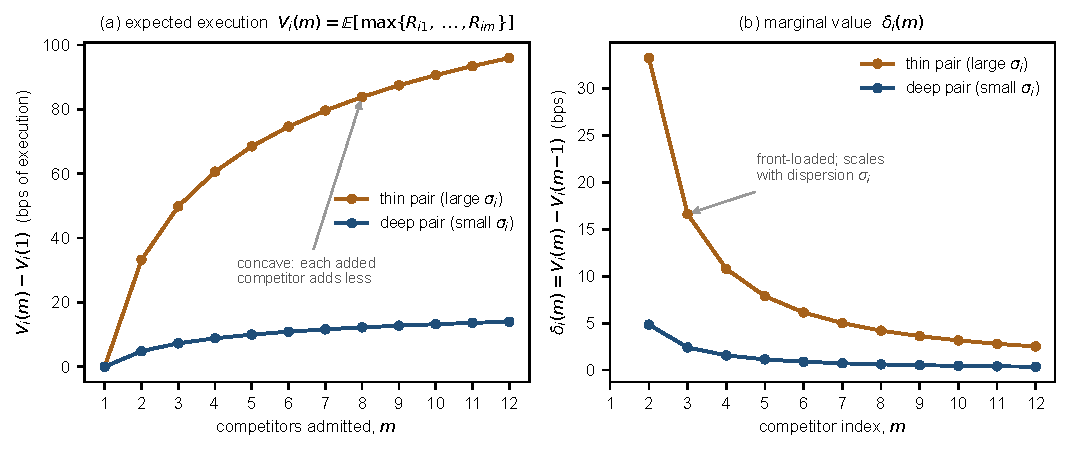
\includegraphics[width=\linewidth]{figures/fig_model.pdf}
\caption{The model's two core objects, computed from the model of Section~\ref{sec:model-value} (expected maxima of i.i.d.\ capacities) at two dispersion levels. \textbf{(a)} The expected-execution curve $V_i(m)=\E[\max\{R_{i1},\dots,R_{im}\}]$ rises and is concave in the field size $m$, its increments shrinking (Proposition~\ref{prop:diminishing}). \textbf{(b)} The marginal-value curve $\delta_i(m)=V_i(m)-V_i(m-1)$ falls toward zero and, at every $m$, sits higher for the thin pair, whose capacities disperse more (large $\sigma_i$; Proposition~\ref{prop:dispersion}). The functional shape is illustrative (a normal $G$); the two scales $\sigma_i$ are chosen so the magnitudes resemble the paper's deep and thin strata.}
\label{fig:model}
\end{figure}

\subsection{Entry, rewards, and the participation channel}\label{sec:model-entry}
Participation is endogenous, so the field size in Propositions~\ref{prop:diminishing}--\ref{prop:dispersion} is itself set by the reward rule. Bidding on an order costs $c>0$ (infrastructure, computation, inventory reservation). A solver's expected gross rent in a field of $m$ is its win probability times the expected reward margin; write it $\pi_i(m;\rho)$, a function of the field size and the reward schedule $\rho$. Free entry pins equilibrium participation $n^\ast_i(\rho)$ at the marginal entrant's zero-profit point,
\begin{equation}\label{eq:entry}
\pi_i\big(n^\ast_i;\rho\big)\;=\;c .
\end{equation}
This is the costly-entry auction of \citet{mcafee1987entry} and \citet{levin1994entry}, whose zero-profit equilibrium already routes the seller's instruments through the participation margin; the entry-cost oligopoly that \citet{chitra2024intent} predict for intent venues is the same economics on-chain. Combining \eqref{eq:entry} with the marginal-value curve delivers the reform prediction.

\begin{proposition}[Participation channel]\label{prop:neutrality}
Suppose bids are approximately invariant to the reward level, as the runner-up-keyed schedule of Assumption~\ref{ass:truth} encourages. Then a reward change $\rho\to\rho'$ moves realized execution quality only through equilibrium participation, and to first order
\begin{equation}\label{eq:channel}
\Delta Q_i \;\approx\; \delta_i\!\big(n^\ast_i\big)\,\Delta n^\ast_i,
\qquad \Delta n^\ast_i := n^\ast_i(\rho')-n^\ast_i(\rho),
\end{equation}
the marginal-value curve of Proposition~\ref{prop:diminishing} evaluated at the participation change the reform induces.
\end{proposition}
\begin{proof}
Under bid invariance the reward enters the model only through the free-entry condition \eqref{eq:entry}, where a higher expected reward supports a larger $n^\ast_i$ at fixed cost $c$. Realized quality is $V_i(n^\ast_i)$ up to the fixed-bid mapping, so a first-order expansion gives $\Delta Q_i\approx V_i'(n^\ast_i)\,\Delta n^\ast_i=\delta_i(n^\ast_i)\,\Delta n^\ast_i$. The runner-up-keyed reward makes bid invariance reasonable but not exact (Assumption~\ref{ass:truth}), so \eqref{eq:channel} is a benchmark to test, not a theorem.
\end{proof}

\begin{remark}[Conditional invariance]\label{rem:invariance}
The idealized model has a sharper corollary: the bid distribution, and hence the runner-up margin conditional on $n$, is invariant to the reward level. I state it for completeness but do not treat it as testable in field data, because $n$ is an equilibrium object and order composition co-moves with membership (Section~\ref{sec:discussion}). Section~\ref{sec:time} tests Proposition~\ref{prop:neutrality} instead through a cross-sectional exposure design the mechanism itself supplies, exploiting that the capped reward weakens truthfulness exactly where the cap binds~\citep{cowdao_rewards}.
\end{remark}

Proposition~\ref{prop:neutrality} states \emph{where} a reward reform acts (membership and participation) and \emph{how much} quality can move (the curve times the induced participation change), which is the level at which identification exists. The decomposition has a named ancestry: \citet{li2009entry} separate auction policy into an entry effect and a competition effect, and \citet{athey2011open} split format effects into participation and bidding-margin components; in a second-score venue the competition effect on bids is nil under truthfulness, isolating the entry effect. A symmetric comparative static covers exits: removing draws from the maximum lowers realized execution and re-entry restores it, a substitution prediction whose fixed-bid version Section~\ref{sec:exitstudy} tests against realized outcomes. In the spirit of \citet{bulow1996auctions}, though not as a test of their theorem, whose symmetric private-values premises this market does not meet, the model says a venue gains more from one additional serious competitor than from refining its allocation rule; Section~\ref{sec:results} reports the field magnitudes relevant to that comparison.

\section{Data}

\subsection{The venue}\label{sec:venue}
CoW Protocol clears trades in discrete auctions. The protocol collects signed intents into a batch, broadcasts the batch to a permissioned but open set of bonded solvers, receives competing settlement proposals, and selects winners under the fair combinatorial auction it adopted on 20~June 2025 (CIP-67): solvers submit bids on individual orders and on batches, the best individual-order bids define a reference outcome per directed token pair, and batched bids that would leave any trade worse than its reference are filtered out~\citep{cowdao_rules,cowdao_fairauction}. Winning solvers are rewarded by a second-price-flavoured rule keyed to the margin of their score over the runner-up's, subject to caps~\citep{cowdao_rewards}. On 8~December 2025, inside my sample window, governance proposal CIP-74 re-tied the reward cap to protocol revenue and introduced a volume-based fee, repricing participation without changing the allocation rule~\citep{zhang2026incentives}. Critically for this paper, the protocol publishes the entire solver-competition record for every auction, all submitted solutions, winning and losing, with solver identities, proposed per-order executions, and a native price vector valuing every token in ETH~\citep{cow_api}. By contrast, the per-order Dutch auctions of UniswapX and 1inch Fusion~\citep{adams2023uniswapx} disclose no losing quotes, which is why this measurement is possible only here. My data sample begins after the combinatorial auction went live, so the allocation mechanism is held fixed throughout except for the CIP-74 reward change I study directly.

\subsection{The data sample}\label{sec:data}
The data sample instantiates the model's primitives of Section~\ref{sec:model-setup}: each record is an order $i$, the set of solvers that competed for it, and the execution ratio each offered, so the ranked offers of Section~\ref{sec:panel} are the empirical image of the capacities $R_{ij}$. I collect every settlement auction on Ethereum mainnet from 12~August 2025 to 15~August 2026: 565{,}259 auctions containing 692{,}964 settled orders quoted against USDC. Restricting to USDC-quoted orders fixes a common numeraire and retains roughly half of the venue's flow: in a random sample of auctions, 53 percent of orders (standard error 1.5) are quoted against USDC, the single most common numeraire on CoW. Orders are stratified by a liquidity metric computed from the data sample itself: each counter-asset's total ETH volume over the sample, on a log scale, cut into asset quintiles L1 (thinnest) through L5 (deepest). Because volume concentrates in few assets, the deepest quintile carries most orders; per-quintile composition appears in Table~\ref{tab:field}. An auxiliary dataset completes the record: for 509{,}309 of the roughly 590{,}000 distinct executed orders (the 692{,}964 settled orders include re-inclusions of partially-fillable orders across batches) I hold a counterfactual quote from the Uniswap smart-order router, pinned to the order's settlement block, together with per-block base fees to net out the direct-swap gas a settled user avoids. The remainder trade tokens for which the router returns no path, long-tail assets without a Uniswap market, so a direct-route counterfactual does not exist for them; this coverage limit mildly favors more liquid assets in any result that uses the routed benchmark. Realized price improvement against that benchmark is the realized-quality outcome of the experiments in Section~\ref{sec:results}. Block heights are approximated to calendar time by a linear model anchored at the data sample's first and last block timestamps, a fair approximation given Ethereum's fixed twelve-second slot schedule.

\subsection{The bid panel}\label{sec:panel}
The observed bids of the model (Section~\ref{sec:model-setup}) are constructed as follows. For each order $i$ in each auction I extract, from every submitted solution, the execution each solver proposed for that order, and keep each solver's best proposal, yielding the ranked offers $r_i^{(1)}\ge\dots\ge r_i^{(n_i)}$ of \eqref{eq:ranked} with their solver identities. Two sanity filters guard against non-economic records: offer gaps are winsorized at 2{,}000 basis points, binding on 0.09 percent of orders, and notionals whose native-price valuation exceeds $10^5$~ETH are treated as missing. Figure~\ref{fig:anatomy} shows one representative auction: twelve solvers competed for a one-ETH WETH/USDC order, the field's bids cluster within a few basis points of the best losing bid, and the runner-up margin (Definition~\ref{def:gap}) is about one basis point, competition at work in its normal, healthy state. Table~\ref{tab:field} in Section~\ref{sec:results} reports the panel's participation structure.

\begin{figure}[t]
\centering
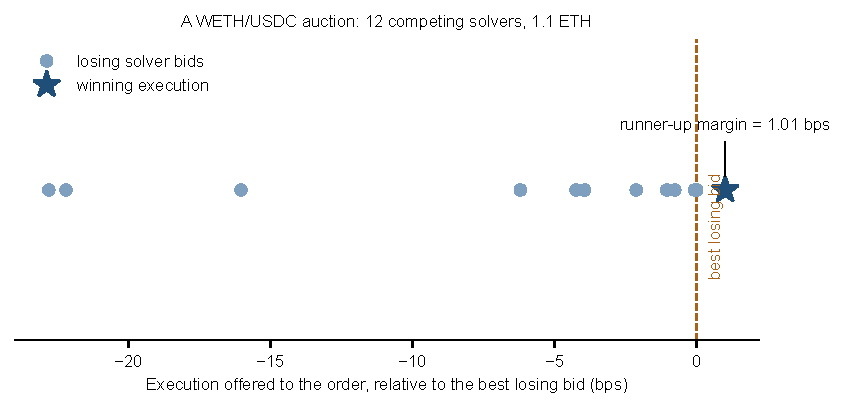
\includegraphics[width=\linewidth]{figures/fig_anatomy.pdf}
\caption{Anatomy of one auction from the data sample: the bids of twelve competing solvers for a single 1.07~ETH WETH/USDC order, expressed relative to the best losing bid. The winning execution (star) exceeds the best losing bid by a runner-up margin of 1.0 basis points; the remaining field sits within a few basis points, with one distant outlier. Every element of the figure is on the public record.}
\label{fig:anatomy}
\end{figure}

\begin{table}[t]
\centering
{\fontsize{10}{12}\selectfont
\begin{tabular}{lr}
\toprule
Stage & Count \\
\midrule
Solver-competition records in the data sample & 565{,}259 \\
\quad with a settled USDC-quoted order & 552{,}234 \\
Settled order instances (USDC-quoted) & 692{,}964 \\
\quad distinct executed orders & 589{,}987 \\
\quad with a routed AMM counterfactual & 509{,}309 \\
Orders with $\ge 2$ competitive bids (margin defined) & 532{,}102 \\
Balanced panel, $\ge 5$ bids & 380{,}387 \\
\quad after 1\% single-bid-value trim (estimand panel) & 376{,}583 \\
\bottomrule
\end{tabular}}
\caption{Sample flow, from the full data sample to the balanced panel underlying the marginal-value estimand, in exact final counts. Settled order instances exceed distinct executed orders because partially-fillable orders re-enter across batches; the routed AMM counterfactual exists only for tokens with a Uniswap market (Section~\ref{sec:data}).}
\label{tab:flow}
\end{table}

\subsection{Empirical objects and their theoretical content}\label{sec:model-objects}
The model's objects map onto the bid panel without estimation. Fix an order with $n_i$ recorded offers, ranked $r_i^{(1)}\ge r_i^{(2)}\ge\dots\ge r_i^{(n_i)}$. The expected best offer among a uniformly random subset of $m\le n_i$ of its solvers is exact, and is the empirical counterpart of $V_i(m)$ in \eqref{eq:Vm} conditional on the realized field:
\begin{equation}\label{eq:subset}
\widehat V_i(m) \;:=\; \sum_{k=1}^{n_i} r_i^{(k)}\,\frac{\dbinom{n_i-k}{\,m-1\,}}{\dbinom{n_i}{\,m\,}},
\end{equation}
where the weight is the probability that the $k$-th ranked offer is the best of a random $m$-subset (the ranks below $k$ furnish the other $m-1$ members); the weights are hypergeometric and sum to one. The order-level \emph{competition-depth counterfactual} and its first difference are
\begin{equation}\label{eq:delta}
\Delta_i(m) \;:=\; 10^4\,\frac{r_i^{(1)}-\widehat V_i(m)}{r_i^{(1)}}\ \text{(bps)},
\qquad
\delta_i(m) \;:=\; \Delta_i(m{-}1)-\Delta_i(m),
\end{equation}
the quality the order forgoes, relative to its full observed field, when only $m$ of its competitive bids are admitted, and the marginal value of the $m$-th admitted bid, the fixed-field analogue of $\delta_i(m)$ in \eqref{eq:Vm}. Both hold the recorded bids fixed; $\Delta_i(m)$ is a mechanical, design-based quantity, not a causal treatment effect. The runner-up margin $\Delta_i$ of Definition~\ref{def:gap} is the boundary case $m=n_i{-}1$ restricted to removing the single best bidder, and aggregating notional-weighted runner-up margins by the identity of the best bidder yields each solver's \emph{fixed-bid exposure}, the user loss its absence alone would impose.

Each theoretical result maps to a designated test. The concavity of the curve (Proposition~\ref{prop:diminishing}) and its liquidity ordering (Proposition~\ref{prop:dispersion}) are read from the pooled $\Delta_i(m)$ and its shape across liquidity quintiles, on the balanced panel of orders with $n_i\ge 5$, with pooled mean and median and auction-clustered bootstrap intervals (Section~\ref{sec:curve}). The exit static and the participation channel of Proposition~\ref{prop:neutrality} are tested against realized price improvement in Sections~\ref{sec:exitstudy} and~\ref{sec:time}, precisely where the fixed-bid reading can fail and so is checked rather than assumed. The truthfulness argument of Section~\ref{sec:model-setup} is what licenses reading these objects as competition counterfactuals. The remove-one-solver operation is itself not novel, the protocol computes such a reference score whenever it settles rewards~\citep{cowdao_rewards}; the contribution is deploying the full family $\{\Delta_i(m)\}_{m=1}^{n_i}$ as measurement.

\section{Empirical Results}\label{sec:results}
The results trace one storyline through the model's two curves: competition's value is real and front-loaded, largest where liquidity is thin, and carried by the depth of the field rather than the identity of any solver. Section~\ref{sec:field} describes the field the curves are drawn on. Section~\ref{sec:curve} traces the order-level curve $\Delta_i(m)$ and its liquidity ordering, the direct tests of Propositions~\ref{prop:diminishing} and~\ref{prop:dispersion}, and Section~\ref{sec:shape} recovers the standardized law $G$ behind the curve's shape. Section~\ref{sec:pivotal} turns to the concentration of exposure that share statistics miss. Sections~\ref{sec:exitstudy} and~\ref{sec:time} then confront the fixed-bid reading with the market's own experiments, the December churn and the CIP-74 reform, the tests of the participation channel of Proposition~\ref{prop:neutrality}.

\subsection{The competitive field}\label{sec:field}
Table~\ref{tab:field} describes participation along the liquidity metric. The typical order attracts five to six competing solvers, out of 47 distinct solvers that ever made a best or second-best offer and 22 to 28 active in any given month. Participation is monotone in liquidity: the median order draws 2 bidders in the thinnest asset quintile and 5 in the deepest (means 2.3 and 5.8), and the median runner-up margin falls twentyfold along the same axis, from 48 to 2.4~bps. The p10--p90 ranges show a heavy right tail everywhere: even in the deepest quintile, one order in ten owed its best solver more than 20~bps. Competition is thinnest exactly where the model expects it to matter most. Single-bid orders are common in every quintile, 23 to 48 percent, but they are not further evidence of thinness: the solo share falls monotonically with order size, from 44 percent in the smallest size decile to 13 in the largest, a decline that holds inside deep and thin assets alike (37 to 14 percent within the deepest quintile). Uncontested orders are dust that solvers do not compete over, not evidence of thin markets.


\begin{table}[t]
\centering
{\fontsize{10}{12}\selectfont
\begin{tabular}{lrrrrrr}
\toprule
 & & \multicolumn{2}{c}{Bidders per order} & & \multicolumn{2}{c}{Runner-up margin (bps)} \\
\cmidrule(lr){3-4}\cmidrule(lr){6-7}
Liquidity & orders & median & p10--p90 & solo (\%) & median & p10--p90 \\
\midrule
L1 (thinnest) & 843     & 2 & 1--5  & 47.8 & 48.36 & 4.1--416.4 \\
L2            & 1{,}753  & 3 & 1--6  & 28.1 & 19.67 & 2.4--147.2 \\
L3            & 5{,}403  & 3 & 1--8  & 27.6 & 11.10 & 1.0--99.6 \\
L4            & 26{,}065 & 4 & 1--9  & 24.5 & 6.98  & 0.7--52.0 \\
L5 (deepest)  & 658{,}900 & 5 & 1--12 & 23.1 & 2.39  & 0.2--20.0 \\
\bottomrule
\end{tabular}}
\caption{The competitive field, by liquidity quintile (L1 thinnest to L5 deepest, asset quintiles of the metric of Section~\ref{sec:data}; CoW mainnet data sample, Aug.~2025--Aug.~2026; 692{,}964 settled USDC-quoted orders; 47 solvers ever at first or second rank). ``Solo'' is the share of orders receiving exactly one offer. The runner-up margin (Definition~\ref{def:gap}) is defined on orders with at least two bidders; each variable is reported as its median with the p10--p90 range. Volume concentrates in few assets, so the deepest quintile carries 95 percent of orders.}
\label{tab:field}
\end{table}

\subsection{The marginal value of competition}\label{sec:curve}
Table~\ref{tab:shortfall} reports the paper's central object: the per-order competition-depth counterfactual $\Delta_i(m)$ of Section~\ref{sec:model-objects}, the value forgone by admitting only $m$ of an order's observed competitive bids, computed on the balanced panel of 376{,}583 orders with at least five bidders (the top percentile of single-bid values trimmed). Admitting one random bid leaves the median order 13.9~bps below its full field (mean 23.8, the skew-sensitive reference); a second closes most of that ($\delta(2)=8.3$~bps at the median, 13.7 at the mean), a third adds 2.6, a fourth 1.3, a fifth 0.8. Auction-clustered bootstrap intervals are tight (Table~\ref{tab:shortfall}) because the panel is large. That $\Delta(m)$ declines is mechanical, since the expected maximum over larger subsets of a fixed ranked vector cannot fall; the findings are the magnitudes and the front-loading, the first admitted bid recovering more than half of the single-bid value and later bids adding little.

The curve is ordered by liquidity at every point (Figure~\ref{fig:liquidity}): the single-bidder value of competition rises monotonically as the volume-based liquidity measure falls, from 14~bps at the median in the deepest quintile to 24, 30, and 38 in the next three. Unlike the decline in $m$, this ordering is not mechanical, since the curves could cross at any $m$ and never do. The thinnest quintile (L1) holds only 97 balanced-panel orders; I treat its level (a much larger figure) as descriptive rather than a headline estimate and report the robust gradient across L2--L5. Competition is worth most where execution technologies disagree most, which is where liquidity is thinnest, and precisely there the field is thinnest too (Table~\ref{tab:field}): the market's weakest point is a coincidence of high marginal value and low participation.


\begin{figure}[t]
\centering
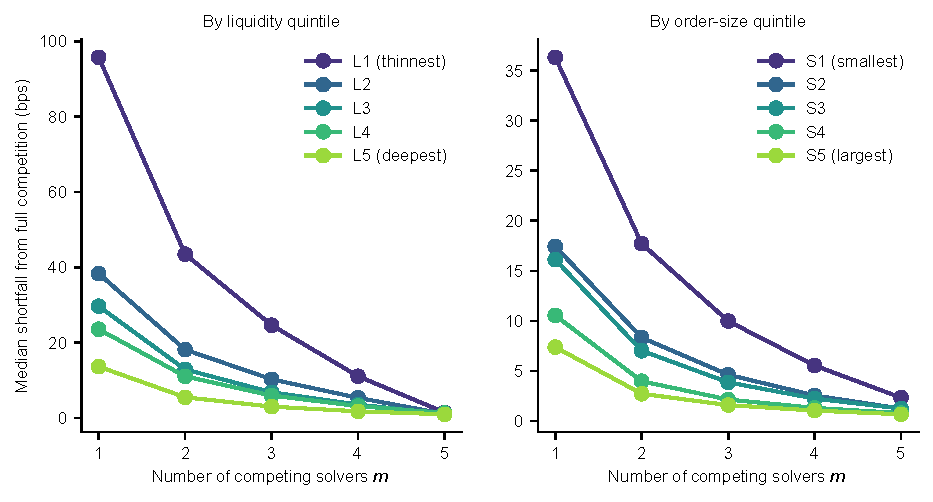
\includegraphics[width=0.92\linewidth]{figures/fig_liquidity.pdf}
\caption{The marginal value-of-competition curve along its two axes. Median competition shortfall $S(m)$, computed exactly per order (Eq.~\eqref{eq:subset}), by liquidity quintile of the counter-asset (left, L1 thinnest to L5 deepest) and by order-size quintile (right, S1 smallest to S5 largest); balanced panel of orders with $n \ge 5$ bidders, top 1\% of single-bidder shortfalls per group trimmed. Bids are held fixed throughout; the decline in $m$ is mechanical, while the magnitudes and the monotone ordering along both axes are the findings. The thinnest liquidity quintile (L1) contains only 97 balanced-panel orders; its level is descriptive, and the robust gradient is across L2--L5.}
\label{fig:liquidity}
\end{figure}

\begin{table}[t]
\centering
{\fontsize{10}{12}\selectfont
\begin{tabular}{lccccc}
\toprule
$\Delta(m)$, bps & $m=1$ & $m=2$ & $m=3$ & $m=4$ & $m=5$ \\
\midrule
\multicolumn{6}{l}{\emph{Value forgone at $m$ admitted bids, pooled (median [95\% CI])}} \\
median & 13.9 & 5.6 & 3.1 & 1.8 & 1.0 \\
       & \tiny[13.9,\,14.0] & \tiny[5.6,\,5.6] & \tiny[3.0,\,3.1] & \tiny[1.8,\,1.8] & \tiny[1.0,\,1.0] \\
mean   & 23.8 & 10.1 & 5.8 & 3.6 & 2.1 \\
       & \tiny[23.6,\,23.9] & \tiny[10.0,\,10.1] & \tiny[5.8,\,5.8] & \tiny[3.5,\,3.6] & \tiny[2.1,\,2.1] \\
\midrule
\multicolumn{6}{l}{\emph{Marginal value of the $m$-th admitted bid, $\delta(m)$ (median [95\% CI])}} \\
median & --- & 8.3 & 2.6 & 1.3 & 0.8 \\
       & & \tiny[8.3,\,8.3] & \tiny[2.5,\,2.6] & \tiny[1.3,\,1.3] & \tiny[0.8,\,0.8] \\
mean   & --- & 13.7 & 4.3 & 2.2 & 1.4 \\
       & & \tiny[13.6,\,13.8] & \tiny[4.2,\,4.3] & \tiny[2.2,\,2.2] & \tiny[1.4,\,1.5] \\
\bottomrule
\end{tabular}}
\caption{The marginal value of competition depth. For each order, $\Delta_i(m)$ is the counterfactual quality forgone by admitting only $m$ of its observed competitive bids (Eq.~\eqref{eq:subset}), in basis points; $\delta(m)$ is its first difference, the value of the $m$-th admitted bid. Reported as pooled mean and median with auction-clustered percentile-bootstrap 95\% confidence intervals (400 replicates resampling the 343{,}675 auctions of the balanced $n\ge5$ panel, 376{,}583 orders; top 1\% of single-bid values trimmed). Intervals are tight because the panel is large; they are not treatment-effect intervals. Per-quintile curves appear in Figure~\ref{fig:liquidity}.}
\label{tab:shortfall}
\end{table}

Order size is the curve's second axis (Figure~\ref{fig:liquidity}, right panel): across order-size quintiles the median single-bidder shortfall falls monotonically from 36.3~bps for the smallest orders to 7.4 for the largest, and the gradient survives inside liquidity groups, from 20.8 to 8.0~bps within the deepest assets and from 75.1 to 23.9 within the second-thinnest. Small orders face material single-bidder exposure even where liquidity is deepest. The runner-up margin tells the same story in the cross-section, falling from 18.3~bps in the smallest size decile to about 1.1 in the largest while participation rises from 5.3 to 8.7 bidders.

\subsection{Recovering the shape of competition}\label{sec:shape}
The curve of Section~\ref{sec:curve} is nonparametric: $\Delta_i(m)$ is computed order by order without a distributional assumption. But the model writes its slope as $\delta_i(m)=\sigma_i\,d_G(m)$ (Proposition~\ref{prop:dispersion}), so the curve's \emph{shape} is governed by a single object, the standardized capacity law $G$ of \eqref{eq:capacity}, and $G$ is itself recoverable from the data. Because each order is an $n_i$-sample of the same $G$, standardizing every order's offers by its own location and scale, $z_{ij}=(r_{ij}-\bar r_i)/s_i$, and pooling across the 67{,}375 orders with $n_i\ge 8$ (775{,}833 offers) traces $G$ out. What is recovered is the shape of \emph{admitted} offers, selected and shaped by the runner-up-keyed reward, not the latent technology; under Assumption~\ref{ass:truth} the two coincide.

The recovered $G$ is not normal (Figure~\ref{fig:shape}). It is strongly left-skewed, with a sample skewness near $-1$: offers pile up just below the best achievable execution, with a long tail of worse offers beneath. Fitting candidate location-scale families by maximum likelihood, the normal is decisively rejected---worse than the best fit by roughly $10^5$ in AIC---while a left-skewed law fits far better: the skew-normal minimizes AIC and the minimum (reversed) Gumbel is close behind, the two families that put a short upper tail and a long lower one exactly where the data do. No parametric law passes a formal goodness-of-fit test at this sample size, so the claim is the shape, not an exact parametric truth: competition among solvers is left-skewed, its upper tail short because offers saturate against the best route. That short upper tail is what makes the marginal-value curve steep. The fitted $G$ implies a normalized marginal-value curve $d_G(m)/d_G(2)$ of $1,\,0.42,\,0.25,\,0.17$ for $m=2,\dots,5$, more front-loaded than the normal benchmark's $1,\,0.50,\,0.33,\,0.24$ and in the direction of the data's own $1,\,0.31,\,0.16,\,0.11$ (Table~\ref{tab:shortfall}); the residual gap is the heterogeneity in $\sigma_i$ that a single pooled $G$ cannot carry. The diminishing-returns result is therefore not an artifact of a normal assumption: a normal $G$ would \emph{understate} how fast competition's value is exhausted.

\begin{figure}[t]
\centering
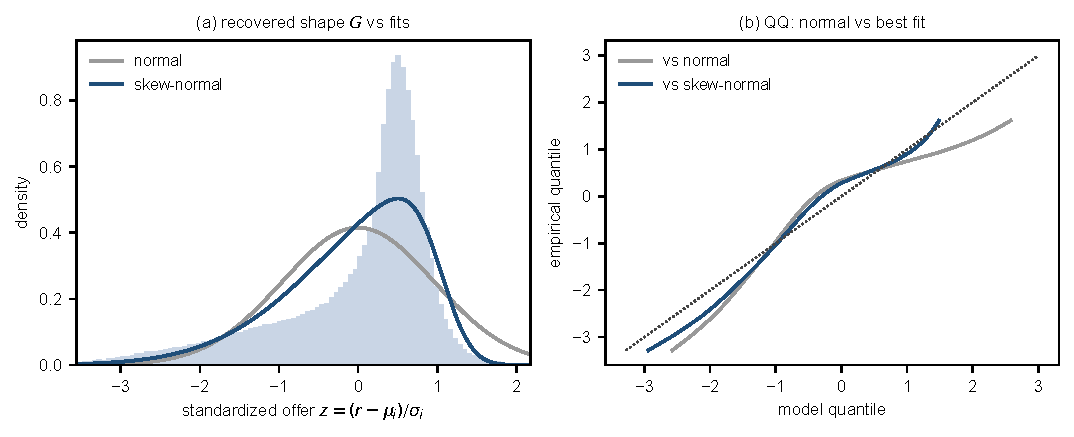
\includegraphics[width=\linewidth]{figures/fig_shape.pdf}
\caption{The recovered shape of competition. \textbf{(a)} The pooled distribution of within-order standardized offers $z=(r-\mu_i)/\sigma_i$ (histogram) is sharply left-skewed; the maximum-likelihood skew-normal (solid) tracks it, the normal (grey) does not. \textbf{(b)} Quantile--quantile plot against the fitted skew-normal and against the normal: the skew-normal hugs the $45^\circ$ line, the normal departs in both tails. Orders with $n_i\ge 8$ from the USDC data sample; the recovered law is the shape of admitted offers.}
\label{fig:shape}
\end{figure}

\subsection{Niche leadership and the concentration of exposure}\label{sec:pivotal}
Who provides this value on the recorded bids? For each order I attribute the runner-up margin to the solver making the best offer, weight by order notional, and aggregate (Section~\ref{sec:model-objects}). Over twelve months this aggregate fixed-bid exposure, the user loss if, order by order, the best bidder had been absent with all other bids unchanged, is about 2{,}586~ETH. Its distribution across solvers is stark (Figure~\ref{fig:pivotal}): the top solver carries 44.5 percent while being best on 53{,}615 orders at a median margin of 2.0~bps; the top two carry 62.4 percent, the top three 69.0. The Herfindahl of this exposure, 0.244, substantially exceeds the Herfindahl of best-offer volume, 0.147. The two indices measure different objects, who would be missed against who wins, and the comparison shows the first is far more skewed than the second, a dimension of market structure that share-based statistics, the only ones the prior literature could compute, do not capture. Whether this measured exposure translates into realized dependence is exactly the question Section~\ref{sec:exitstudy} puts to an experiment, and the answer there qualifies this subsection's reading. A caveat applies to all best-offer-based objects: the winning execution occasionally sits below the order's best recorded offer, so the recorded best offer slightly overstates what the order realized; the realized-quality outcomes used in Sections~\ref{sec:exitstudy} and~\ref{sec:time} are measured on executions and are unaffected.

\begin{figure}[t]
\centering
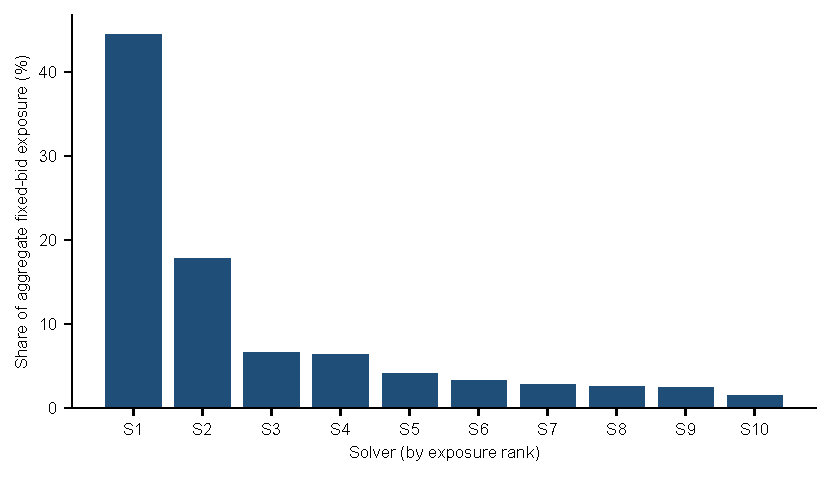
\includegraphics[width=0.88\linewidth]{figures/fig_pivotal.pdf}
\caption{Concentration of fixed-bid exposure. Each solver's share of the aggregate notional-weighted runner-up margin (the user loss its individual absence would impose, holding all other bids fixed), top ten solvers of 47. The top two solvers carry 62 percent of measured exposure; Section~\ref{sec:exitstudy} tests whether such exposure translates into realized dependence.}
\label{fig:pivotal}
\end{figure}

\subsection{Does exposure bind? Substitution through the December churn}\label{sec:exitstudy}
Whether the fixed-bid measure captures realized dependence is a question the market itself answered when the field churned in December 2025; this subsection uses the churn to check the measure, and Section~\ref{sec:time} takes up the reform that plausibly caused it. The field's movements let the data speak without holding bids fixed (Figure~\ref{fig:cip74}). Across the thirteen sample months, the median bidder count and the median runner-up margin co-move with correlation $-0.73$. The sharpest movement is a December 2025 wave of three solver exits, arriving in the effective month of the CIP-74 reward reform and plausibly part of its repricing (Section~\ref{sec:time}): the median field thinned from six bidders in November to three at the February trough while the monthly median margin widened from 2.0 to 4.3~bps, and a wave of entries between February and April 2026, six solvers crossing the activity threshold, rebuilt the field to eight bidders by August and compressed the margin to 1.4~bps. The widening into the trough, about 2.3~bps, is close to what Table~\ref{tab:shortfall}'s within-order curve implies for thinning a five-bidder field to three, 2.1~bps. I read this as consistency between the fixed-bid measure and market dynamics, not as causal identification, because the aggregate series has no control group. The cross-section supplies one.

\begin{figure}[t]
\centering
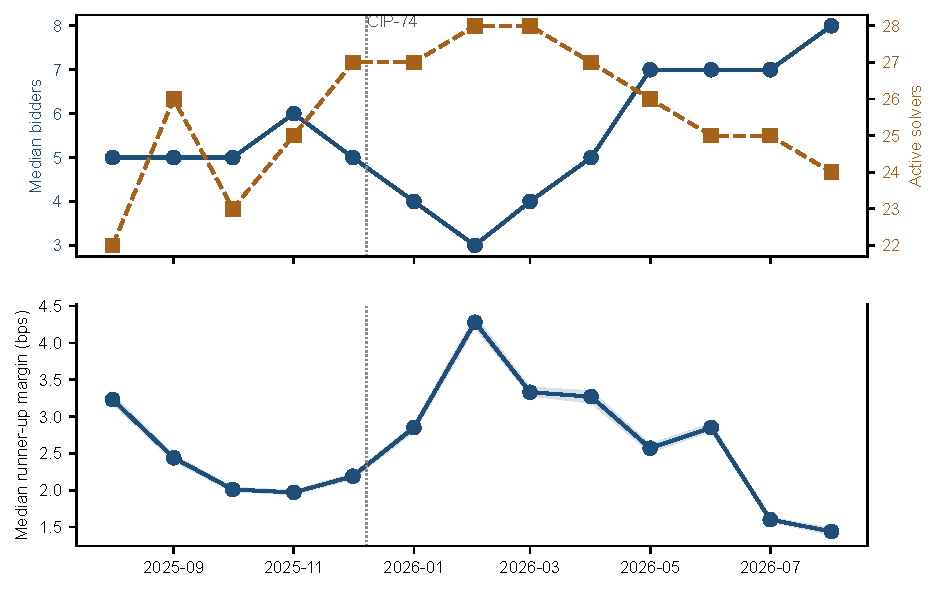
\includegraphics[width=0.95\linewidth]{figures/fig_cip74.pdf}
\caption{Competition and prices over time. Top: median bidders per order (solid, left axis) and active solvers per month (dashed, right axis). Bottom: monthly median runner-up margin. Dotted line: CIP-74 (8~December 2025). The December 2025 exit wave and the spring 2026 entry wave move participation and margins in opposite directions; the monthly correlation between median bidders and median margin is $-0.73$.}
\label{fig:cip74}
\end{figure}


If the fixed-bid exposure measure of Section~\ref{sec:pivotal} captured realized dependence, the counter-assets where the exiting solvers had been most often best should have deteriorated most. I test this directly. The three exiters were, in the three pre-exit months, the best or second-best bidder on 16 percent of all orders; exposure varies sharply across counter-assets, from over 90 percent for the most exposed to essentially zero. I define treated assets as those with at least 25 percent pre-exit top-two exposure (48 assets, median exposure 42 percent) and controls as those below 5 percent (270 assets), on a counter-asset by month panel with equal asset weights. Outcomes are the mean bidder count, the median realized price improvement of executed orders against a routed AMM counterfactual pinned to each order's settlement block (winsorized at $\pm 100$~bps), and the median runner-up margin; the specification removes counter-asset and liquidity-stratum-by-month fixed effects, with strata recut as quintiles of the liquidity metric over the analysis assets so each stratum holds treated and control assets, and standard errors clustered by counter-asset.

The result is a precisely estimated absence of any differential effect, and it is informative. In the three impact months the treated assets lost \emph{no} bidders relative to controls ($-0.05$, standard error $0.18$), realized price improvement did not differentially fall ($-0.9$~bps, standard error $4.7$), and the runner-up margin did not differentially widen ($+1.9$~bps, standard error $2.6$); the event-time paths (Figure~\ref{fig:exitstudy}) are flat through the episode, with no pre-trend and no break. Losing solvers that had been top-two bidders on nearly half of a treated asset's orders left no detectable mark on that asset relative to others. Substitution absorbed the exits at the asset level: remaining and newly entering solvers filled the vacated top-of-field positions within the granularity of a month. Meanwhile the aggregate field thinned and aggregate margins widened, and no asset class escaped it, which is exactly what the cross-section implies when the treatment is near-universal in intensity and individual suppliers are replaceable.

Two conclusions follow, and they sharpen rather than weaken the paper's message. First, the fixed-bid exposure measure of Section~\ref{sec:pivotal} is an \emph{upper bound} on realized dependence: it prices what would be lost if bids stood still, and the experiment shows bids do not stand still, at least not within exposed assets over monthly horizons. Second, what binds is the aggregate depth of the field, not the identity of any solver. Competition matters; competitors are replaceable. The market's exposure is to the participation level itself, which did fall for a quarter, market-wide, until entry restored it.

\begin{figure}[t]
\centering
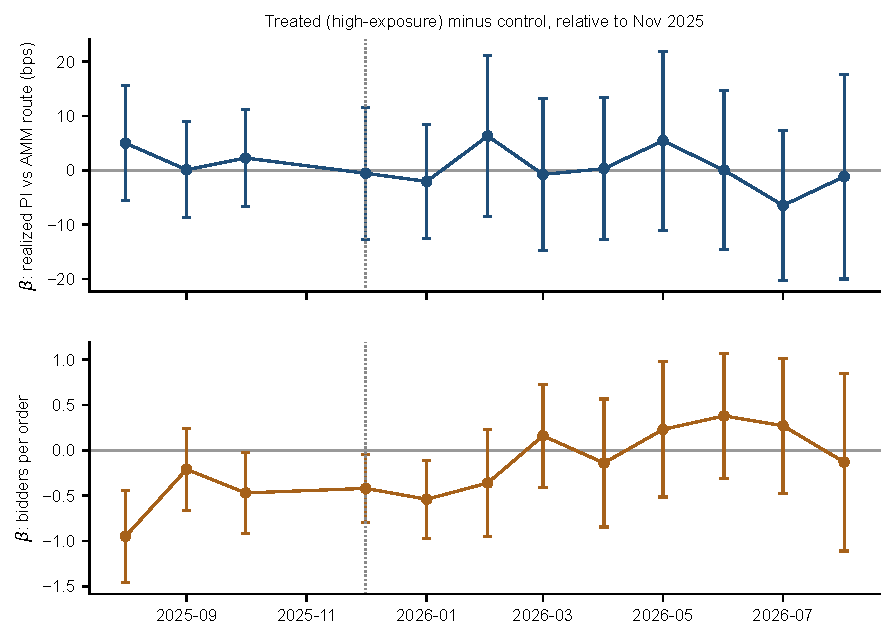
\includegraphics[width=0.92\linewidth]{figures/fig_exitstudy.pdf}
\caption{The exit experiment. Event-time differences between treated (high-exposure) and control counter-assets, relative to November 2025, with 95 percent confidence bands: realized price improvement against the routed AMM counterfactual (top) and bidders per order (bottom). Counter-asset and liquidity-stratum-by-month fixed effects; standard errors clustered by counter-asset. Assets most exposed to the December exiters show no differential deterioration in either outcome.}
\label{fig:exitstudy}
\end{figure}

\subsection{Institutional validation: CIP-74}\label{sec:time}
CIP-74 offers an institutional validation rather than a clean natural experiment: a governance-dated, real-world repricing of solver rewards whose observed patterns are directionally consistent with the participation-channel prediction of Proposition~\ref{prop:neutrality}. I do not claim identification of a treatment effect. The membership churn just documented is timing-consistent with that channel doing the responding: the three exits and three entries of December land in the reform's effective month, and the entry wave that rebuilt the field follows within a quarter. I read the exits as plausibly a response to the repriced rewards, though motives are unobservable in these data. The proposition's two halves then both check out at the level where identification exists. Participation moved, active solvers rising from 23.6 to 26.2 per month and the single-bid share falling from 24.5 to 22.3 percent; and the predicted transmission to quality is small, the net participation change of about a quarter-bidder per order times the curve's $\delta$ near $n=6$ giving well under one basis point, comfortably inside the seven-basis-point bound that \citet{zhang2026incentives} estimates independently. His study reads the same reform through value capture and concentration; this one reads it through participation and margins, and the two are complements on one event.

The conditional-invariance corollary of Remark~\ref{rem:invariance} admits no direct test, for reasons the discussion summarizes; the mechanism itself supplies the test that works, and specifies it in advance. The pre-reform cap was fixed at 0.012~ETH per auction, truthfulness weakens exactly where the cap binds, and CIP-74 replaced it with a revenue-tied cap, so any bid-shading response to the reform should concentrate in assets whose auctions ran into the old cap. In the pre-reform months, 4.5 percent of orders sat in cap-binding auctions, single-winner auctions whose winner--runner-up solution score exceeded the cap. Classifying counter-assets by their pre-reform share of such orders and running the same asset-by-month design as Section~\ref{sec:exitstudy} (109 exposed assets against 121 zero-exposure controls), bidding margins show no differential response: $+1.7$~bps (standard error 4.5) in the transition and $+5.5$ (6.1) thereafter, and $+0.6$ under either halving or doubling of the cap threshold. Participation instead rose differentially in the previously cap-bound assets, $+0.8$ bidders per order (standard error 0.2), which is where the revenue-tied cap raises maximum rewards, the participation channel operating cross-sectionally, though an imperfect pre-trend keeps this reading suggestive. Realized price improvement in exposed assets declines after the reform, but exposure is classified from the same window as the pre-period outcome, so level reversion contaminates that coefficient and I do not interpret it. On its specified object the test is clean: no detectable bidding-margin response to the repricing, consistent with Proposition~\ref{prop:neutrality} and with truthful bidding surviving the reform.

\section{Discussion}\label{sec:discussion}

\paragraph{One law of motion} The results are many, but they obey a single law: in this market, every adjustment runs through the participation margin. The curve prices the depth of the field, and depth is what moves prices, monthly bidder counts and margins co-moving at $-0.73$. Exposure to individual solvers looked like the vulnerability, two firms carrying 62 percent of it and exposure concentration exceeding share concentration, yet when the most-relied-upon solvers left, substitution erased the difference between exposed and unexposed assets within a month. A reward reform reshuffled membership and recruited bidders where the new cap pays more, while bids themselves did not respond. What the market cannot substitute away is aggregate depth: the median field thinned from six bidders to three for a quarter and the monthly median margin roughly doubled until entry rebuilt it, and in the thinnest quintiles, where the residual shortfall at two bidders runs 18 to 43~bps against 5.5 in the deepest, a thin field costs most. For the entry-cost oligopoly the theory predicts~\citep{chitra2024intent}, the empirical price tag attaches to the oligopoly's depth, not its membership. Competition matters; competitors are replaceable.

\paragraph{A caution on conditional comparisons} A natural test of Remark~\ref{rem:invariance} would hold the bidder count fixed and compare margins across reward regimes, and it fails for an instructive reason: $n$ is an equilibrium object. Which orders end up with a given number of bidders changes as membership churns, so conditional-on-$n$ margins mix bidding behavior with order composition. In these data they widen at low $n$ during the transition, then sit below pre-reform levels at low $n$ and above them at high $n$ once the field is rebuilt, and behave no more consistently when restricted to the eleven solvers active throughout; the pattern rejects nothing and confirms nothing. It is why the cap-exposure design of Section~\ref{sec:time}, which varies the incentive rather than conditioning on the outcome, is the test the mechanism supports.

\paragraph{What on-chain transparency teaches, and what it exports} The measurement was possible only because an on-chain venue publishes what every market keeps hidden, and the lessons run in both directions. Toward traditional finance, the law and the curve attach field magnitudes to debates it has conducted largely on theory. Read through the economics of information, the measured curve is Stigler's value-of-search schedule~\citep{stigler1961information}; price-dispersion studies measured its endpoints and the winner--runner-up gap from collected quotations~\citep{pratt1979price,baye2004price}, and this paper, to my knowledge for the first time, draws the whole schedule at every $m$ from a fixed order's observed field. In the spirit of \citet{bulow1996auctions}, though not as a test of the theorem, whose symmetric private-values hypotheses this market does not satisfy, the curve prices what recruiting one more serious bidder is worth, several basis points at the thin end, while the one observed reform of the reward rules was followed by little movement in quality. The winner--runner-up margins are rents in the auction-theoretic sense, a median 2 basis points for the top solver and 3 to 5 in thin assets; whether they are the informational rents of \citet{biais2000competing} the data cannot say. The dealer-competition evidence gains a candidate reconciliation rather than a resolution: here, where bids are sealed and rewards are runner-up-keyed, counts and margins move together tightly, whereas on NASDAQ thirty dealers under continuous visible quoting sustained wide spreads~\citep{christie1994nasdaq}, a pattern consistent with the count measuring competition only jointly with the mechanism. And the December episode refines the slow-moving-capital narrative~\citep{duffie2010capital,grossman1988liquidity} in an unexpected direction: capacity reallocated across assets within a month while aggregate capacity took a quarter to rebuild, locating the friction in building competitive solvers, not in deploying existing ones.

\paragraph{How much competition is enough} The curve gives the question a quantitative answer. In this auction environment the marginal value of competition falls steeply after the first several independent competitors: by around the fifth bid the median order gains well under a basis point from an additional one. This is a statement about the observed sample, not a universal sufficiency threshold. Since the bid record is public and the computation deterministic, any observer, a user, a venue, a supervisor, can recompute the number of independent offers an order received and locate it on the curve. Where best execution is a regulated duty owed by an intermediary~\citep{mifid2,finsa,finra5310}, the duty's functional substitute in a broker-free market is competition, and the law of motion says exactly which statistic to watch: the aggregate depth of the field, an informative and publicly recomputable screen, though not a proven sufficient statistic, since its informativeness rests on the mechanism keeping bids competitive, which this paper maintains as an idealization and disciplines with two experiments rather than establishes. This gives concrete content to the argument that verifiable execution can stand in for conduct regulation~\citep{le2026fairness}: what should be verified is not only the winning price but the depth of the field behind it, and the verification is a direct computation on published data.

\paragraph{Design and entrants} The results tell designers where their levers are. Reward parameters moved participation, not bids, so a venue that wants better thin-market execution, where a single-bidder field forgoes tens of basis points at the median in the thinnest quintiles, gains most from whatever recruits and retains marginal bidders there. For entrants, the runner-up margins are the invitation: they price the rent available to a firm with genuine execution capacity precisely where the field is thin, and the substitution result is the entrant's reassurance and the incumbent's warning in equal measure. I leave the business-model economics to future work; the map of where competition is scarce is drawn here.

\subsection{Policy implications}\label{sec:policy}
The measurement is positive rather than normative, but three implications for auction design follow directly from the magnitudes, offered as design guidance disciplined by the estimates rather than as identified causal effects. All three exploit the fact that makes the measurement possible: the field behind each order is published and the curve is recomputable, so a designer can act on the very statistic the participation law singles out.

\paragraph{Weight rewards toward shallow fields, not volume} The curve is steep at its start and flat by its end (Table~\ref{tab:shortfall}): a fifth or sixth bid on a deep pair is worth well under a basis point to the median order, while a second bid in the thinnest quintile is worth tens. A reward rule that tracks volume therefore spends most of its budget where the marginal competitor is nearly worthless and little where it is worth the most, because volume concentrates in the deep pairs that are already contested. Tilting the reward toward low-depth auctions and thin counter-assets---paying more for participation precisely where the field is shallow---buys more execution quality per unit of reward than any uniform increase. The reform evidence is consistent with this lever having force: CIP-74 moved participation, not conditional bids (Section~\ref{sec:time}), and the cap-exposure test recruited bidders where the new cap paid more, so reward parameters act on who shows up, which is what the thin end needs.

\paragraph{Floor the single-bidder auction against a public benchmark} A single-bid field is the configuration the curve prices most dearly: relative to a full field the median solo order forgoes about fourteen basis points, and more in thin assets. Many solo orders are small trades that solvers rationally leave uncontested (Section~\ref{sec:field}), which bounds the aggregate cost, but that is no comfort to the thin-asset orders where a solo field and a large penalty coincide. A venue cannot conjure a second solver on demand, yet it can bound the damage when none arrives, by requiring the winning solution to improve on a mechanical reserve---the routed on-chain AMM price this paper already computes for every order as its realized-quality benchmark (Section~\ref{sec:data}). Such a floor turns ``one bid or nothing'' into ``one bid, no worse than the public route,'' capping the left tail of solo execution without touching contested auctions, where the winner beats the reserve anyway. The reserve is undefined for the long-tail assets that have no Uniswap market---the same coverage limit the benchmark carries here---so it protects the thin-but-routable orders it can price and leaves the truly illiquid ones to disclosure.

\paragraph{Publish the field-depth screen as a live execution statistic} Where best execution is a regulated duty owed by a broker, a broker-free venue's functional substitute is competition, and aggregate field depth is the statistic the participation law says to watch. Because the bid record is public and the computation deterministic, the venue can expose that statistic continuously: the depth-one penalty by liquidity bucket---the median value a solo order forgoes against the full field---recomputed order by order and reported as a standing series. This operationalizes the argument that verifiable execution can substitute for conduct regulation~\citep{le2026fairness}: what a supervisor, a user, or the venue itself should verify is not only the winning price but the depth of the field behind it, and unlike any screen a traditional venue could publish, this one is a direct computation on already-public data.

\subsection{Robustness and limitations}\label{sec:limits}

\paragraph{Robustness} The estimand carries auction-clustered percentile-bootstrap intervals (Table~\ref{tab:shortfall}); they are narrow because the panel holds 376{,}583 orders across 343{,}675 auctions, so sampling uncertainty is small relative to the reported magnitudes. The liquidity gradient is the robust object: it is monotone across the four populated quintiles L2--L5, whose balanced samples are large, and does not depend on the thinnest quintile L1, which contains only 97 balanced-panel orders and enters as descriptive material. The institutional-validation reading of CIP-74 (Section~\ref{sec:time}) is supported by two independent designs, the exit-exposure contrast and the pre-specified cap-exposure test, and by the independent execution-quality bound of \citet{zhang2026incentives}; none is offered as clean causal identification.

Five limitations bound the claims. First, the fixed-bid counterfactuals rest on a maintained idealization. Bids-as-capacities is motivated by the runner-up-keyed reward, but the production mechanism's caps and batch selection blunt the argument, and the exit experiment shows directly that participation adjusts; the cap-exposure test finds no bidding-margin response to the reform, which supports the idealization but is a bounded null, not proof, so the thinning curve should be read as an exact statement about the recorded field and an upper bound on equilibrium dependence. Second, a per-order proposal inside a batch solution need not be independently feasible once other orders change, so batch coupling qualifies not only bidding incentives but the feasibility of the counterfactual assignments themselves. Third, participation is endogenous: solvers choose which orders to bid on, so cross-sectional comparisons of $n$ conflate order attractiveness with competition, which is why the headline objects are within-order computations and the identified result is a designed contrast rather than a regression on $n$. Fourth, the data sample covers one venue, one chain, one quote asset, and only settled orders; the fill-rate series uses an expiry-based date proxy, and selection into settlement is not modeled. This is not incidental, since no other venue publishes losing bids, but it means external validity rests on the model, not the data: the curve's shape and the substitution finding are hypotheses for other markets, while the levels are this market's own. Fifth, solver identity is an on-chain address. If one operator runs several addresses, measured exposure concentration understates true concentration; the substitution result is robust in the reassuring direction, since consolidation would make the absorbed exits larger, not smaller, but the exposure rankings themselves carry the caveat.

\section{Conclusion}

What is one more competitor for a customer order worth? For fifty years the question could only be answered by inference, because the bids that lose are unobserved in every market that debated it. The first production market I know of to publish them permits a design-based answer computed from the record: order by order, the value forgone when fewer competitive bids are admitted, holding observed bids fixed. That value is large, quickly exhausted, and unevenly supplied. Admitting one bid instead of the full field costs the median order about 14 basis points; a second closes most of the gap; by around the fifth the marginal gain is under a basis point in this sample; and the value is largest where liquidity is thinnest. Measured exposure is concentrated in two firms. Yet when three major solvers left in December 2025, the assets most exposed to them fared no worse than others, while the monthly median margin roughly doubled for a quarter as the field thinned and then recovered through entry; and around the CIP-74 reward reform, membership churned and participation moved while margins conditional on participation changed little. These patterns, which I read as institutional validation rather than clean identification, point one way: adjustment runs through the depth of the field, not the identity of its members, so the design-based measure is an upper bound on realized dependence. Competition matters, competitors are replaceable, and in markets that have replaced the broker's duty with an auction, the depth of the field, publicly recomputable order by order, is where investor protection now lives.

\section*{Acknowledgement}

This research received no external funding.

\section*{Author Contributions}

N.B.\ is the sole author and performed all aspects of the study: conception, data collection, analysis, and writing.

\section*{Conflict of Interest}

The author declares no conflict of interest.

\bibliographystyle{unsrtnat}
\bibliography{references}

\end{document}
